\section{Fresh Replication and Action
Content}\label{fresh-replication-and-action-content}

\begin{longtable}[]{@{}llrrrr@{}}
\caption{Fresh replication and action-remapping control, ten paired
training seeds per setting. Bank-versus-none gains are significant in
five settings, excluding MultiRoom Count-PPO. Bank-versus-remapped gains
are significant in all six settings and positive in all sixty pairs.
Means are rounded independently.}\tabularnewline
\toprule\noalign{}
Task & Student & None AUC & Bank AUC & Remapped AUC & Bank final (\%) \\
\midrule\noalign{}
\endfirsthead
\toprule\noalign{}
Task & Student & None AUC & Bank AUC & Remapped AUC & Bank final (\%) \\
\midrule\noalign{}
\endhead
\bottomrule\noalign{}
\endlastfoot
DoorKey-8 & PPO & .023 & .937 & .000 & 98.4 \\
DoorKey-8 & Count-PPO & .444 & .995 & .945 & 100.0 \\
MultiRoom-N6 & PPO & .000 & .738 & .000 & 86.0 \\
MultiRoom-N6 & Count-PPO & .960 & .992 & .556 & 100.0 \\
KeyCorridor-S3R3 & PPO & .000 & .828 & .000 & 99.4 \\
KeyCorridor-S3R3 & Count-PPO & .936 & .995 & .916 & 100.0 \\
\end{longtable}

The content control remaps each action by a fixed permutation,
\((a+3)\bmod6\). Applicability and abstention are unchanged for a given
state. Training trajectories and realized advice exposure may differ
between arms. Original targets improve on the remapped targets in every
setting, but the remapped targets themselves improve DoorKey Count-PPO
over no advice. The control therefore supports the importance of action
content without claiming that all gains require correct targets.

\begin{figure}
\centering
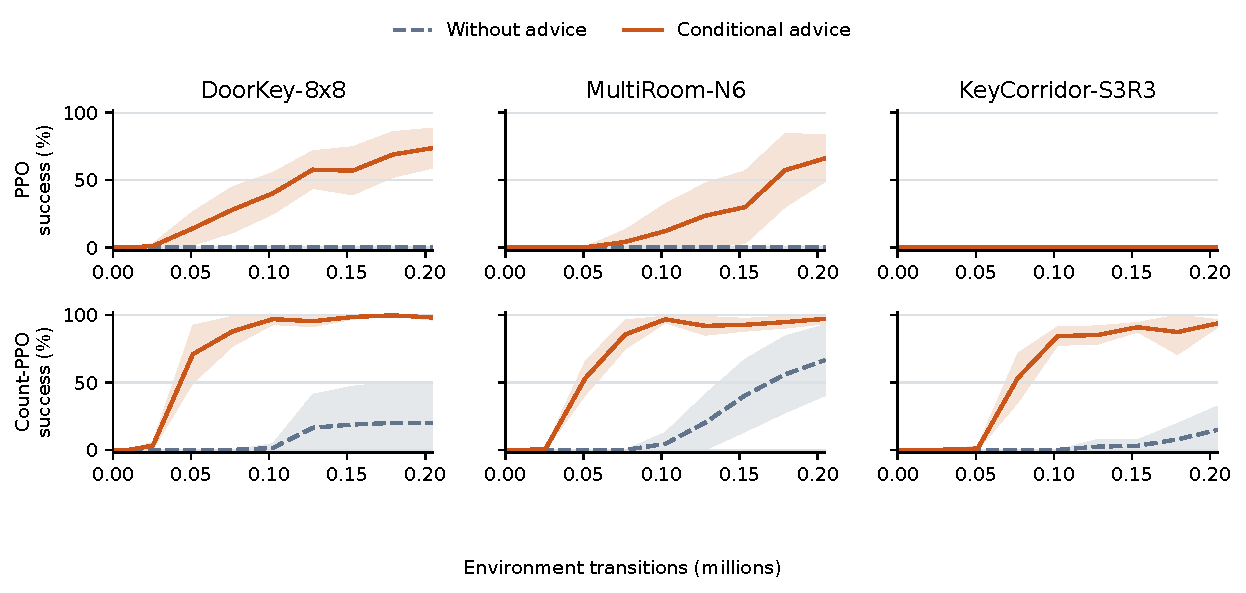
\includegraphics[width=1\linewidth,height=\textheight,keepaspectratio,alt={Fresh-cohort early greedy success on an ordinary linear axis, including measured initialization. Each panel uses ten training seeds per arm.}]{figures/source_fresh_early_greedy.pdf}
\caption{Fresh-cohort early greedy success on an ordinary linear axis,
including measured initialization. Each panel uses ten training seeds
per arm.}
\end{figure}

\begin{figure}
\centering
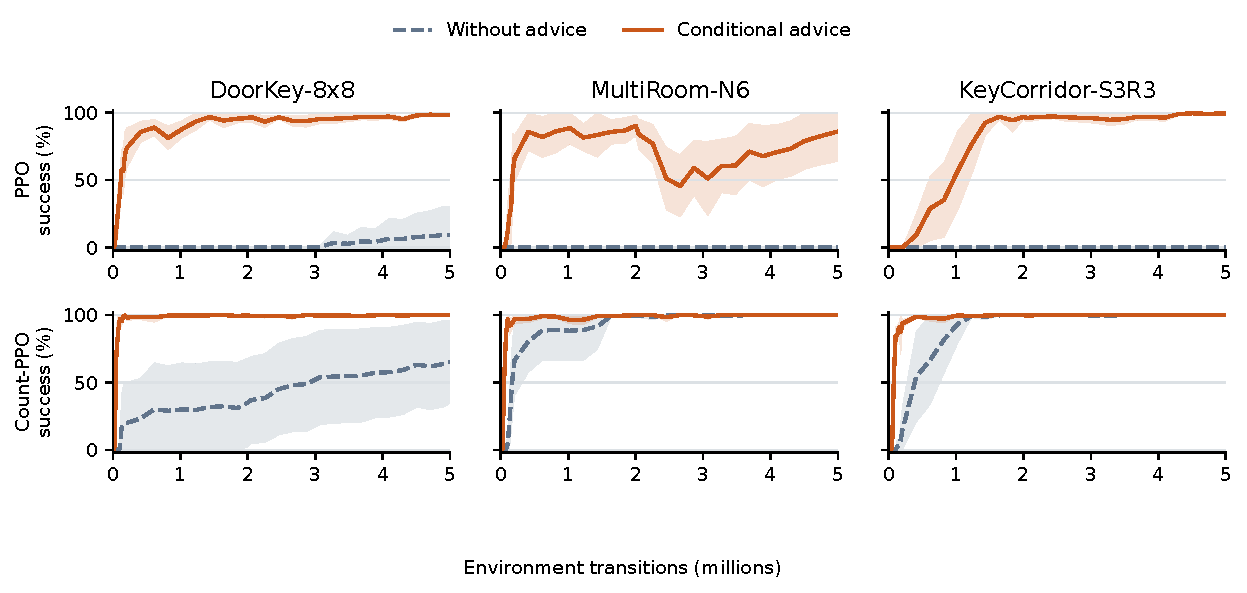
\includegraphics[width=1\linewidth,height=\textheight,keepaspectratio,alt={Fresh-cohort greedy success over the full training budget on a linear axis.}]{figures/source_fresh_linear_greedy.pdf}
\caption{Fresh-cohort greedy success over the full training budget on a
linear axis.}
\end{figure}

\begin{figure}
\centering
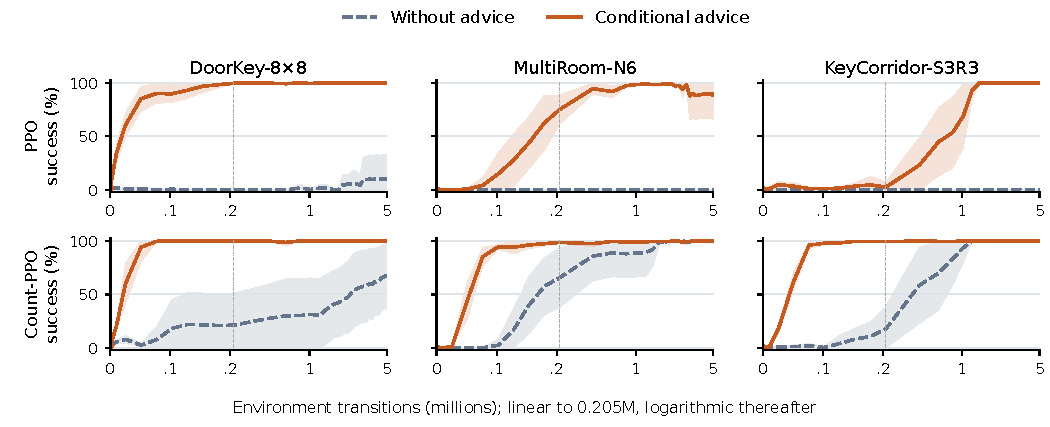
\includegraphics[width=1\linewidth,height=\textheight,keepaspectratio,alt={Sampled-action success on the same fresh cohort as the initialization diagnostics.}]{figures/source_fresh_sampled.pdf}
\caption{Sampled-action success on the same fresh cohort as the
initialization diagnostics.}
\end{figure}




The original confirmation-cohort sampled curves, including no advice, appear
in the main paper's combined four-method figure. The figures here retain
the fresh-cohort initialization measurements and are not spliced into that comparison.
